\documentclass[conference,a4paper]{IEEEtran}
\IEEEoverridecommandlockouts
\usepackage[utf8]{inputenc}
\usepackage[T1]{fontenc}
\usepackage{cite}
\usepackage{amsmath}
\usepackage{graphicx}
\usepackage{booktabs}
\usepackage{array}
\usepackage{url}
\usepackage[hidelinks]{hyperref}
\makeatletter
\newcommand{\linebreakand}{\end{@IEEEauthorhalign}\hfill\mbox{}\par\mbox{}\hfill\begin{@IEEEauthorhalign}}
\makeatother
\def\BibTeX{{\rm B\kern-.05em{\sc i\kern-.025em b}\kern-.08em
    T\kern-.1667em\lower.7ex\hbox{E}\kern-.125emX}}

\begin{document}

\title{HeatGuard: An AI-Based Early Warning System for Heat Stress in Outdoor Workers Using Simulated IoT Wearables}

\author{
\IEEEauthorblockN{Zayed Zanober}
\IEEEauthorblockA{ID 8417386}
\and
\IEEEauthorblockN{Faseeh Padinjarathil}
\IEEEauthorblockA{ID 8418779}
\and
\IEEEauthorblockN{Jaanvi Chugani}
\IEEEauthorblockA{ID 9959877}
\and
\IEEEauthorblockN{Rayen Chaouachi}
\IEEEauthorblockA{ID 1268806}
\and
\IEEEauthorblockN{Fahmi Shafeeq}
\IEEEauthorblockA{ID 8982569}
\linebreakand
\IEEEauthorblockA{Faculty of Engineering and Information Sciences, University of Wollongong in Dubai, Dubai, United Arab Emirates\\ CSIT305 Emerging Technology Research and Innovation Project}
}

\maketitle

\begin{abstract}
HeatGuard is a browser-based early-warning prototype that estimates whether a simulated outdoor worker will reach a core-temperature threshold within 30 minutes. We compared five policies on identical simulated shifts: the UAE midday break alone and the break combined with a Heat Index rule, Thermal Work Limit (TWL), Wet Bulb Globe Temperature (WBGT), or HeatGuard. The simulator combined the ISO 7933 Predicted Heat Strain model with worker variability and self-pacing on ERA5 Dubai weather. A logistic regression was trained on 200 virtual workers in 2025 weather and tested once on 100 different virtual workers in 2024 weather (4,000 shifts, 720 events). HeatGuard missed 8 events versus 5 for WBGT, meeting the pre-registered 2-percentage-point sensitivity margin in this run. HeatGuard averaged 163 warning minutes per shift versus 493 for WBGT, a 67\% reduction. The warning reduction persisted across exploratory checks, while the sensitivity margin failed under higher worker variability and in one smaller repeat. The experiment evaluates alert performance in simulation. Field validation on UAE workers remains open.
\end{abstract}

\begin{IEEEkeywords}
heat stress, early warning, wearable sensors, Internet of Things, machine learning, occupational safety, UAE
\end{IEEEkeywords}

\section{Introduction}

\subsection{Background}
Occupational heat exposure harms health and limits work capacity \cite{kjellstrom}. The UAE midday-break policy restricts work outdoors in direct sun from 12:30 to 15:00, 15 June to 15 September \cite{mohre}. Dubai's guideline puts the high-risk Heat Index band at 40--45 \textdegree C \cite{dm}, while Abu Dhabi's code calls for a process using TWL to determine work--rest breaks and water needs \cite{oshad}, \cite{brake}. ISO describes WBGT-based screening and NIOSH provides exposure limits \cite{iso7243}, \cite{niosh}. UAE companies have trialled wearables \cite{ega}, but a review of 96 studies found limited field validation of occupational heat technologies \cite{asto}.

\subsection{Problem Statement and Stakeholders}
The calendar break applies during fixed hours and dates. Environmental rules can account for workload and acclimatisation, but do not directly observe each worker's changing physiological response. HeatGuard tests whether simulated wearable signals help distinguish workers approaching the study's danger threshold while limiting warning time.

\subsection{Research Question and Contributions}
\textbf{RQ:} In a Dubai-weather simulation, can a worker-specific warning model retain sensitivity within a pre-set margin of Heat Index, TWL and WBGT rules while reducing warning burden? The contribution is a reproducible paired comparison and a browser artefact with a supervisor board, worker display and sensor-fault fallback.

\section{Related Work and Research Gap}

\subsection{Rule-Based Heat Stress Assessment}
WBGT and its workload-dependent exposure limits are widely used \cite{iso7243}, \cite{niosh}. TWL was derived from heat balance and evaluated with UAE construction workers \cite{brake}, \cite{millerbates}, \cite{bates}. In a US case series, WBGT-based limits were exceeded in 22 of 25 occupational heat illnesses \cite{tustin}. In a separate agricultural study, WBGT risk levels often exceeded the strain indicated by an individual physiological index \cite{sousan}. These studies motivate measuring both misses and warning burden.

\subsection{Wearables and Machine Learning}
Hirata et al.\ estimated core temperature from wearable and environmental inputs \cite{hirata}. Moyen et al.\ evaluated a non-invasive Kenzen temperature estimate \cite{moyen}. Shimazaki et al.\ used personalised vital signs for occupational heat prediction \cite{shimazaki}, Ojha et al.\ used physiological signals and ensemble learning \cite{ojha}, and Choi et al.\ forecast personal allowable exposure time \cite{choi}.

\subsection{Research Gap}
These studies establish wearable-based estimation and prediction. They leave the operational trade-off open for this setting: whether worker-specific alerts retain sensitivity relative to site rules while reducing warning time and false episodes. We study that trade-off using a locked paired comparison on simulated shifts, with missed events, lead time, false episodes and warning minutes as outcomes.

\section{Method}

\subsection{Research Design}
We ran a paired simulation experiment. Every option sees the same weather, workers and schedule, and a separate body model provides the reference outcome. Warnings do not change the simulated day, so all options are scored against the same counterfactual. The frame, hypotheses, margin and verdict rule were signed off, and the plan committed to the repository, before the test set was scored in a single locked run.

\subsection{Weather}
Hourly ERA5 reanalysis \cite{era5}, retrieved through the Open-Meteo archive \cite{openmeteo}, for the Dubai grid cell (25.0\textdegree N, 55.25\textdegree E), 1 June to 30 September, for 2025 (training) and 2024 (locked test). Hourly values were interpolated to minutes. WBGT was computed with the Liljegren method \cite{liljegren} in thermofeel \cite{thermofeel} and the Heat Index with the NWS Rothfusz formula \cite{rothfusz}. Mean radiant temperature was assumed to be air temperature $+10$\,\textdegree C in exposed work and $+1$\,\textdegree C in shade.

\subsection{Simulated Workers}\label{sec:workers}
The day runs 06:00--18:00 with 45 minutes of work and 15 minutes of shaded rest each hour. From 15 June to 15 September the legal break 12:30--15:00 is in the schedule, with no exposure and no warnings. Workers vary in mass (55--95\,kg), height (1.60--1.90\,m), acclimatisation (balanced) and work rate (100, 165 or 230\,W/m$^2$). Body temperature comes from ISO 7933 Predicted Heat Strain (PHS) \cite{iso7933} in pythermalcomfort \cite{pythermal}, chained minute by minute.

PHS describes a standard person, so we added documented differences between people: a resting core offset (SD 0.2\,\textdegree C), the share of sweat replaced by drinking (assumed 50--90\%; UAE workers stay mildly dehydrated \cite{bates}), and an assumed dehydration gain of 0.10--0.20\,\textdegree C per 1\% body mass lost, informed by \cite{sawka}. Real workers also slow down when hot \cite{selfpacing}: each worker eases to 65\% of their work rate once their core passes their own pace point (mean 37.7\,\textdegree C) and returns 0.15\,\textdegree C lower. These two values were tuned on separate calibration workers so that the share of worker-days passing 38.0, 38.3 and 38.5\,\textdegree C matched 55 Guatemalan field workers \cite{krisher}: 45/18/6\% in our training set against 44/16/6\% in the field.

We had no participant-level UAE worker data for the locked study. Published field summaries provide descriptive comparisons. Against two other studies the simulated workers run hot: they spend 14\% of work time at 38.0--38.4\,\textdegree C against about 3\% in 125 workers in Qatar \cite{qatar}, and their mean working heart rate is 105\,bpm (91 in the lightest work group) against 87--91\,bpm in UAE construction workers studied in May \cite{bates}, at a WBGT of 26--29\,\textdegree C against 33\,\textdegree C in our summer data.

A \emph{danger event} is the first minute during work at which the adjusted rectal temperature reaches 38.2\,\textdegree C (38.5\,\textdegree C if acclimatised); it is a study definition, not a diagnosis. Heart rate, skin temperature and activity are emitted each minute with noise; heart-rate readings outside 30--220\,bpm count as missing.

\subsection{Data Sets}
Training: 200 workers $\times$ 30 random dates of 2025 = 6,000 shifts, 937 events. Locked test: 100 different workers $\times$ 40 random dates of 2024 = 4,000 shifts, simulated before the run and never scored before it.

\subsection{Compared Options}
All options keep the legal break (Table~\ref{tab:options}). Comparators use each worker's own work rate and acclimatisation and are computed every minute, a best case for them. TWL is our own implementation of the published definition \cite{brake}: the highest work rate at which a standard acclimatised worker keeps core temperature $\le$38.2\,\textdegree C and sweat $\le$1.2\,kg/h. Against three published field values \cite{millerbates} it is $-1\%$, $+5\%$ and $+23\%$ off.

\begin{table}[!t]
\caption{Compared Options (All Keep the Legal Break)}
\label{tab:options}
\centering
\footnotesize
\setlength{\tabcolsep}{3pt}
\begin{tabular}{@{}p{0.6cm}p{1.9cm}p{4.9cm}@{}}
\toprule
Code & Option & Warns outside the midday break when \\
\midrule
C1 & Break only \cite{mohre} & Never \\
C2 & + Heat Index & NWS Heat Index \cite{rothfusz} $\ge$ 40\,\textdegree C. The threshold is drawn from \cite{dm}. \\
C3 & + TWL \cite{oshad}, \cite{bates} & TWL $<$ 115\,W/m$^2$ ($<$ 140 if unacclimatised), dry bulb $>$ 44\,\textdegree C or wet bulb $>$ 32\,\textdegree C \\
C4 & + WBGT \cite{niosh} & WBGT above the worker's NIOSH RAL/REL (60-min averages) \\
HG & + HeatGuard & Model risk $\ge$ threshold; WBGT fallback if the HR sensor fails; everyone warned at Heat Index $\ge$ 54\,\textdegree C \\
\bottomrule
\end{tabular}
\end{table}

\subsection{Model and Threshold}
HeatGuard uses logistic regression \cite{sklearn} to predict whether an event starts within 30 minutes. Its 25 inputs are trailing 5- and 15-minute summaries and trends of heart rate, skin temperature and activity; current and 60-minute WBGT and Heat Index; body size, acclimatisation and planned work rate; reading-quality flags; time of day; the pace gap (how much slower than planned the worker moves); and heart-rate and skin-temperature rise above the day's low. All use past or current readings only; core temperature is never an input. Random forest and gradient boosting never met the tuning limit and were dropped.

The threshold and a warning hold (0, 15 or 30 minutes) were chosen out-of-fold across five groups of training workers: among settings whose miss rate is at most the safest index rule's training miss rate plus 1 point, with median lead $\ge$25 minutes, take the fewest false episodes, then the fewest warning minutes. The choice was threshold 0.32 with a 30-minute hold (training: 3.5\% missed, 162 warning minutes per shift). The model was refitted on all training workers and scored once on the test set; no test worker or test year was used for any choice, to avoid leakage \cite{kapoor}.

\subsection{Measures, Hypotheses and Verdict}\label{sec:hyp}
Warnings separated by at least five clear minutes start separate episodes. Events are caught only by warnings in the 30 minutes before onset. Lead time is measured from the earliest such warning, with zero for misses. Warning minutes and episodes are scored before the first event, or through shift end on event-free shifts. Episodes without pre-event overlap are false alarms, with new episodes in the last 30 minutes of event-free shifts excluded from that count. Intervals use 2,000 worker-level bootstrap resamples.

\begin{table}[!t]
\caption{Pre-Registered Hypotheses}
\label{tab:hyp}
\centering
\footnotesize
\begin{tabular}{@{}p{0.45cm}p{2.3cm}p{4.65cm}@{}}
\toprule
 & Claim & Passes if \\
\midrule
H1 & More catches than break alone & HG $-$ C1 sensitivity: interval above 0 \\
H2 & As safe as each index rule & HG $-$ rule sensitivity: lower bound $\ge -2$ points (margin $M=2$) \\
H3 & Far fewer warnings & Warning minutes $\ge$50\% lower (lower bound) and false episodes not higher \\
H4 & Warns as early & Median lead difference: lower bound $\ge -5$ min \\
H5 & Robust to faults & H2 holds with a 10-min HR dropout and a 15-min stuck sensor \\
H6 & Catches what rules miss & $a$ (rule missed, HG caught) $>$ $b$ (reverse), exact one-sided McNemar $p<0.05$ \\
\bottomrule
\end{tabular}
\end{table}

Per rule, HeatGuard wins on \emph{precision-or-safety} if H3 passes or it is clearly safer (sensitivity lower bound above 0). The gap is \emph{closed} if H1 passes, H2 passes against C2--C4, and HeatGuard wins on precision-or-safety against each of them.

\section{The HeatGuard Artefact}

\subsection{Architecture}
The study pipeline has six Python parts (Fig.~\ref{fig:arch}): a weather loader; a worker and shift generator; the PHS body simulator with person-to-person differences and self-pacing; simulated wearables that emit one MQTT-style JSON message per minute (topic \texttt{heatguard/worker/<id>/vitals}); the alert engine; and a scorer. The simulator's core temperature goes only to the scorer, never to the alert engine, so the model cannot see the answer.

\begin{figure}[!t]
\centering
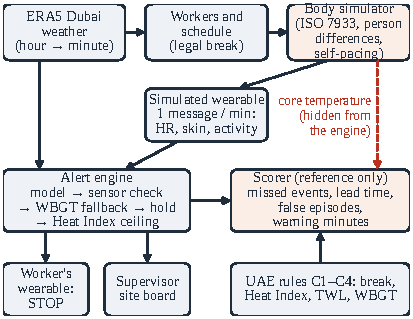
\includegraphics[width=\columnwidth]{fig1.pdf}
\caption{HeatGuard architecture. The observation path (weather and wearables to the alert engine, the worker's wearable and the site board) is separate from the reference path (core temperature to the scorer only).}
\label{fig:arch}
\end{figure}

\subsection{Alert Engine}
Each minute the engine builds its inputs from past and current readings, scores the model and applies four rules in order. (1) \emph{Sensor check}: after two missing heart-rate readings in a row, or five identical ones, the reading is not trusted and the engine falls back to the WBGT rule; if the WBGT rule is unavailable too, it warns. It returns to the model when valid readings resume. (2) \emph{Model warning}: warn when the predicted 30-minute risk is at least 0.32. (3) \emph{Hold}: once on, the warning stays on for 30 minutes after the last trigger, so the wearable does not flicker. (4) \emph{Ceiling and break}: everyone is warned when the Heat Index reaches 54\,\textdegree C (NWS extreme danger, 3\% of 2024 work hours); no warnings are sent during the legal break, when nobody works.

\subsection{Interface}
The warning goes to two people. The worker's wearable shows OK, STOP or REST. The supervisor's site board shows every worker's state, risk and sensor status, and opens any worker minute by minute against the three index rules. For the demonstration the alert engine itself was ported to JavaScript and runs inside one web page, with no installation. The viewer can switch a heart-rate sensor off or freeze it at any minute and watch the fallback, and the page lists the inputs that push the current risk up or down.

\subsection{Testing and Performance}
The Python suite had 46 passes, one expected failure in the Week 7 model and five skips from the empty manual-case fixture. Of 17 AI-proposed edge cases, 15 were implemented and exposed two defects. A hand check reproduced one 30-minute lead time. The independent student-authored comparison remained incomplete. The Python and browser engines agreed on warning and fallback states across 36,720 replay minutes, and eight offline browser checks passed. A dashboard review using Nielsen's heuristics \cite{nielsen} identified the need for clearer sensor-fault status and a multi-worker board, both addressed in the replay. Median decision latency was 12\,ms (95th percentile 14\,ms). The Appendix links to the code, data and reviewer files.

\section{Results}
The locked test was run once on 16 November 2026. It contained 720 danger events: 593 on days when the legal break applied (207 of them in the 15:00 hour, right after the break) and 127 on days outside the break dates. Table~\ref{tab:results} gives the main results with clean sensors and Table~\ref{tab:tests} the hypothesis tests.

\begin{table}[!t]
\caption{Locked Test Results (4,000 Shifts, 720 Events, Clean Sensors)}
\label{tab:results}
\centering
\footnotesize
\setlength{\tabcolsep}{3pt}
\begin{tabular}{@{}lrrrrr@{}}
\toprule
Option & Missed & Sens. & Lead & False/shift & Warn min \\
\midrule
C1 Break only & 720 & 0\% & -- & 0.00 & 0 \\
C2 + NWS Heat Index & 26 & 96.4\% & 30 & 1.53 & 446 \\
C3 + TWL & 559 & 22.4\% & -- & 0.23 & 17 \\
C4 + WBGT & 5 & 99.3\% & 30 & 1.61 & 493 \\
\textbf{HG + HeatGuard} & \textbf{8} & \textbf{98.9\%} & \textbf{30} & \textbf{1.08} & \textbf{163} \\
\bottomrule
\end{tabular}
\end{table}

\begin{table}[!t]
\caption{Hypothesis Tests (95\% Intervals From Resampling Workers)}
\label{tab:tests}
\centering
\footnotesize
\setlength{\tabcolsep}{3pt}
\begin{tabular}{@{}p{1.2cm}p{2.15cm}p{1.75cm}p{2.15cm}@{}}
\toprule
 & vs Heat Index & vs TWL & vs WBGT \\
\midrule
H2 sens. diff. & $+2.5$ pts [$+0.1$, $+5.4$] pass & $+76.5$ pts pass & $-0.4$ pts [$-1.0$, 0.0] pass \\
H3 warn min & $-63\%$ [57, 70] pass & n/a; clearly safer & $-67\%$ [62, 72] pass \\
H4 lead diff. & 0 min pass & $+30$ min pass & 0 min pass \\
H6 $a$ vs $b$ & 21 vs 3, $p=0.0001$ pass & 554 vs 3 pass & 0 vs 3, not passed \\
\bottomrule
\end{tabular}
\end{table}

\textbf{H1.} HeatGuard warned before 98.9\% of events (interval 98.0--99.6\%), against 0\% for the break alone.

\textbf{H2 and H3.} HeatGuard was within the 2-point margin of every rule. Against the NWS Heat Index rule it was more sensitive; against WBGT it missed 3 more events of 720 (0.4 points). Five events began in the first minute after the legal break, when no option can warn; these are all 5 WBGT misses and 5 of HeatGuard's 8. HeatGuard's other three misses occurred in the first 40 minutes of the day. Against both, it cut warning minutes by about two thirds and false episodes by about a third. TWL warned for only 17 minutes per shift but missed 559 events, so HeatGuard had substantially higher sensitivity (Fig.~\ref{fig:tradeoff}).

\begin{figure}[!t]
\centering
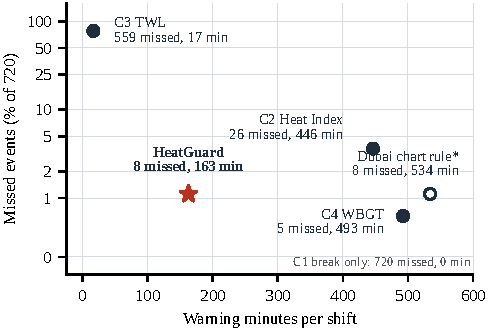
\includegraphics[width=\columnwidth]{fig2.pdf}
\caption{Warning minutes per shift against missed events (log scale), locked test set. *Scored after the locked run (exploratory).}
\label{fig:tradeoff}
\end{figure}

\textbf{H4.} Median lead was 30 minutes for HeatGuard, WBGT and Heat Index alike.

\textbf{H5.} With a 10-minute heart-rate dropout or a 15-minute stuck sensor, HeatGuard still missed 8 events and H2 held. Its warning minutes rose to 207 and 216 per shift and its false episodes to 1.63 and 1.61, level with WBGT. Only 13 events began near the fault window, so this is a weak test.

\textbf{H6.} HeatGuard caught 21 events the NWS Heat Index rule missed (3 the other way, $p=0.0001$) and 554 the TWL rule missed (3 the other way). It added no catches over WBGT (0 vs 3).

\textbf{Verdict.} H1 passed; H2 passed against all three index rules; HeatGuard won on precision-or-safety against each (H3 against Heat Index and WBGT, clearly safer against TWL). Under the pre-registered rule, the research gap is closed.

\subsection{Exploratory Checks After the Locked Run}
These checks were planned and committed after the test set had been seen and before any of them was run. All are reported; none can change the verdict above.

\textbf{Dubai chart approximation.} The locked C2 used the NWS formula. For the exploratory check, Humidex \cite{humidex} reproduced five sampled values from the Dubai lookup chart \cite{dm}. The resulting threshold rule (40 or above) yielded 534 warning minutes per shift and 8 misses, the same miss count as HeatGuard (3 discordant events in each direction). HeatGuard averaged 69\% fewer warning minutes [64, 75]. This is a chart approximation.

\textbf{Alarm burden.} In the scoring window, no warnings appeared on 34\% of HeatGuard shifts (WBGT 0.2\%). HeatGuard averaged 1.08 false episodes per shift versus 1.61 for WBGT.

\textbf{Inputs.} The largest standardised weights were for heart-rate rise above the day's low, pace gap and 5-minute heart rate. After re-tuning on training workers, the variant without wearable inputs missed 56 events at 193 warning minutes per shift. The variant without weather inputs missed 6 at 157 minutes. Removing pace and activity yielded 42 misses at 184 minutes.

\textbf{Stress test and other seeds.} Halving worker variability yielded 616 events and 3 HeatGuard misses (WBGT 1), at 173 warning minutes (WBGT 503). Increasing it by half yielded 890 events and 23 misses (WBGT 11) at 153 minutes (WBGT 479). The sensitivity difference, $-1.3$ points [$-3.1$, $-0.2$], crosses the 2-point margin. Across three 1,000-shift repeats (183, 177 and 133 events), HeatGuard missed 5, 3 and 0 versus 1, 2 and 0 for WBGT, while reducing warning minutes by 66--76\%. One repeat failed the sensitivity margin.

\textbf{After a sensor fault.} A 15-minute stuck sensor left event detection unchanged, but added a median 42 warning minutes and more than 240 on 85 of 4,000 shifts. An unplanned diagnostic on 500 shifts split the extra minutes roughly evenly between fallback and hold, and later warnings associated with a lowered stored heart-rate baseline. The locked model retains this defect.

\textbf{Measured-data follow-up.} Fitting simulated heart-rate recovery to PROSPIE \cite{prospie} reduced held-out error from 6.96 to 6.69\,bpm across five lab participants. Retraining on paired Dubai simulations yielded three misses out of 84 events with either recovery rate. Mean six-hour heart rate was 80.6\,bpm in an Australian mine-worker group trace \cite{taggart} and 100.9\,bpm in the calibrated simulation. These are exploratory comparisons. Validation on measured UAE workers remains open.

\section{Discussion}
\textbf{Interpretation.} Every simulated event occurred outside the scheduled midday break. About 29\% occurred in the first hour after work resumed on break days and 18\% occurred outside the policy dates. WBGT caught the most events in the locked comparison. The TWL implementation warned least and missed the most events among the index rules. HeatGuard met the sensitivity margin with about one third of WBGT's warning minutes. Because warnings never changed the simulated trajectories, the experiment measures detection and warning burden.

\textbf{Failures and iteration.} Our first test (mornings only, WBGT alone) found the model not better: 7 missed events of 26 against 0, with thresholds tuned on as few as 4 events. In the new design the first data set failed its realism check and was discarded unscored; the first tuning target (99\% of training events) was impossible for every model and for the rules themselves; and without a hold the warning flickered. Each change used training data only. After the locked run, a review of our own draft found that C2 was not Dubai's actual rule; the chart approximation above was scored separately.

\textbf{Security, privacy and ethics.} Heart rate and estimated heat strain are health data. A deployment needs informed consent, encrypted device communication and access limited to the worker and the safety officer. The engine needs only the last 60 minutes of readings, so raw data need not be stored, and its outputs must not be used to measure productivity or to discipline workers. The team collected no new participant data. The exploratory analysis used published measurements.

\textbf{Organisational and sustainability implications.} A STOP for one worker only helps if the site can act on it: supervisors need spare capacity, a shaded rest area and a procedure for sensor faults. HeatGuard should complement the break and the index rules, not replace them; the WBGT fallback and the Heat Index ceiling keep a rule-based floor. The model is a 25-input logistic regression that runs in a browser, with the measured decision latency reported in Section IV.

\section{Limitations}
\textbf{Simulated physiology.} ISO 7933 supplied the reference temperature. Simulated heart rate, skin temperature and pace depend on the same body model, so the strongest predictors share assumptions with the outcome. The training results reflect the self-pacing calibration to published field values \cite{krisher}. Ten of 100 test workers account for 55\% of events, and afternoon events depend on the assumed lack of fluid replacement during the midday break.

\textbf{Transfer of measured data.} The PROSPIE work-to-rest heart-rate and rectal-temperature readings from 15 lab participants were used to fit one simulator coefficient controlling the rate of heart-rate recovery. Five participants were held out to check that fit. Both warning models were then trained on paired simulated Dubai shifts, and both missed 3 of 84 events in the exploratory simulation test. Australian summer mine-worker heart-rate and core-temperature readings were used as descriptive benchmarks after training. The higher simulated heart rate and the differences in climate, work and rest schedules limit transfer. The Australian group-average trace cannot establish individual alert accuracy, and field validation on UAE workers remains open.

\textbf{Evaluation assumptions.} Comparators used minute-level workload and acclimatisation. TWL was implemented for this study, and the locked Heat Index rule used the NWS formula. ERA5 was interpolated to minutes and radiant temperature used an assumed offset. Only 13 events occurred near scripted faults, and faults sometimes prolonged warnings. Lead time is capped at 30 minutes. The usability evidence consists of alarm measures and a heuristic review. Two exploratory checks missed the WBGT sensitivity margin.

\section{Conclusion}
On 4,000 held-out simulated shifts, HeatGuard caught 98.9\% of 720 events with a median 30-minute lead. It met the pre-registered WBGT sensitivity margin and reduced warning minutes by 67\%. The reduction persisted in exploratory checks, while sensitivity fell outside the margin under higher worker variability and in one smaller repeat. Future work includes testing faults near event onset, preventing excess warnings after faults, and validating on measured UAE workers.

\appendix[Access to Supplementary Materials]
\noindent\textbf{GitHub}\quad \href{https://github.com/rayen1214-hub/Heatguard}{\underline{github.com/rayen1214-hub/Heatguard}}.\\
\noindent\textbf{SharePoint}\quad \href{https://uowmailedu-my.sharepoint.com/:f:/g/personal/fp418_uowmail_edu_au/IgAwG3WqqWcARrZaE-4lCy9QASuq_GTxz7iU6o4pjrf9EiU?e=v9Q385}{\underline{Open the submission folder}}.

GitHub provides the code, data documentation, tests and reproduction steps. The SharePoint folder provides the paper and offline demo.

\section*{Acknowledgment}
\textit{Declaration of Generative AI Use.} We defined the research question, comparators and evaluation rules. We ran the early simulations and conducted the dashboard usability review. We used Claude Code to generate simulation, analysis and demo code, execute the locked and post-hoc runs, and draft the manuscript. We used ChatGPT and Codex to assist with the usability write-up, measured-data analysis and revisions. We record the sessions and review status in the repository's AI-use log.

\begin{thebibliography}{00}
\bibitem{kjellstrom} T. Kjellstrom, D. Briggs, C. Freyberg, B. Lemke, M. Otto, and O. Hyatt, ``Heat, human performance, and occupational health: A key issue for the assessment of global climate change impacts,'' \emph{Annu. Rev. Public Health}, vol. 37, pp. 97--112, 2016, doi: 10.1146/annurev-publhealth-032315-021740.
\bibitem{mohre} Ministry of Human Resources and Emiratisation, \emph{Occupational Health and Safety Guide}, occupational heat stress prevention policy. \href{https://www.mohre.gov.ae/assets/download/6ef28a8/Occupational-Health-and-Safety-Guide-EN.pdf.aspx}{Official guide}.
\bibitem{dm} Dubai Municipality, \emph{Technical guidelines for management of heat stress at work}, DM-HSD-GU38-MHSW2, ver. 3.0, May 2024. \href{https://www.dm.gov.ae/wp-content/uploads/2024/07/DM-HSD-GU38-MHSW2_Technical-Guidelines-for-Management-of-Heat-Stress-at-Work_V3.pdf}{Official guideline}.
\bibitem{oshad} Abu Dhabi Public Health Centre, \emph{ADOSH-SF Code of Practice 11.0: Safety in the Heat}, ver. 4.0, Jul. 2024. \href{https://www.adphc.gov.ae/-/media/Project/ADPHC/ADPHC/PDF/OSHAD-SF/Codes-of-Practise/11---Safety-in-the-Heat-v31-English.pdf}{Official code}.
\bibitem{brake} D. J. Brake and G. P. Bates, ``Limiting metabolic rate (thermal work limit) as an index of thermal stress,'' \emph{Appl. Occup. Environ. Hyg.}, vol. 17, no. 3, pp. 176--186, 2002, doi: 10.1080/104732202753438261.
\bibitem{iso7243} \emph{Ergonomics of the Thermal Environment---Assessment of Heat Stress Using the WBGT (Wet Bulb Globe Temperature) Index}, ISO 7243:2017, 2017. \href{https://www.iso.org/standard/67188.html}{ISO catalogue}.
\bibitem{niosh} B. L. Jacklitsch \emph{et al.}, ``Criteria for a recommended standard: Occupational exposure to heat and hot environments,'' NIOSH, DHHS Publ. No. 2016-106, 2016, doi: 10.26616/NIOSHPUB2016106.
\bibitem{ega} Emirates Global Aluminium, ``EGA extends use of wearable technology to `Beat the Heat' in the UAE summer,'' Aug. 9, 2023. [Online]. Available: \href{https://media.ega.ae/ega-extends-use-of-wearable-technology-to-beat-the-heat-in-the-uae-summer/}{EGA announcement}
\bibitem{asto} R. F. Asto Bonifacio, B. Y. Buendia Milla, and J. J. Huaman Rojas, ``Predicting occupational heat stress in critical sectors: A sector-based systematic review of wearable sensing, IoT platforms, and machine-learning models,'' \emph{J. Robot. Control}, vol. 6, no. 5, pp. 2152--2165, 2025, doi: 10.18196/jrc.v6i5.27377.
\bibitem{millerbates} V. S. Miller and G. P. Bates, ``The thermal work limit is a simple reliable heat index for the protection of workers in thermally stressful environments,'' \emph{Ann. Occup. Hyg.}, vol. 51, no. 6, pp. 553--561, 2007, doi: 10.1093/annhyg/mem035.
\bibitem{bates} G. P. Bates and J. Schneider, ``Hydration status and physiological workload of UAE construction workers: A prospective longitudinal observational study,'' \emph{J. Occup. Med. Toxicol.}, vol. 3, Art. no. 21, 2008, doi: 10.1186/1745-6673-3-21.
\bibitem{tustin} A. W. Tustin \emph{et al.}, ``Evaluation of occupational exposure limits for heat stress in outdoor workers---United States, 2011--2016,'' \emph{MMWR}, vol. 67, no. 26, pp. 733--737, 2018, doi: 10.15585/mmwr.mm6726a1.
\bibitem{sousan} S. Sousan \emph{et al.}, ``Assessing the feasibility of wearable devices for physiological monitoring and heat risk prediction in outdoor agricultural workers,'' \emph{Am. J. Ind. Med.}, vol. 69, no. 9, pp. 722--744, 2026, doi: 10.1002/ajim.70103.
\bibitem{hirata} A. Hirata \emph{et al.}, ``Body core temperature estimation using new compartment model with vital data from wearable devices,'' \emph{IEEE Access}, vol. 9, pp. 124452--124462, 2021, doi: 10.1109/ACCESS.2021.3110252.
\bibitem{moyen} N. E. Moyen, R. C. Bapat, B. Tan, L. A. Hunt, O. Jay, and T. M{\"u}ndel, ``Accuracy of algorithm to non-invasively predict core body temperature using the Kenzen wearable device,'' \emph{Int. J. Environ. Res. Public Health}, vol. 18, no. 24, Art. no. 13126, 2021, doi: 10.3390/ijerph182413126.
\bibitem{shimazaki} T. Shimazaki, D. Anzai, K. Watanabe, A. Nakajima, M. Fukuda, and S. Ata, ``Heat stroke prevention in hot specific occupational environment enhanced by supervised machine learning with personalized vital signs,'' \emph{Sensors}, vol. 22, no. 1, Art. no. 395, 2022, doi: 10.3390/s22010395.
\bibitem{ojha} A. Ojha, S. Shayesteh, A. Sharifironizi, Y. Liu, and H. Jebelli, ``Worker-centric heat strain analysis: Integrating physiological signals with ensemble learning and domain adaptation,'' \emph{Autom. Constr.}, vol. 166, Art. no. 105670, 2024, doi: 10.1016/j.autcon.2024.105670.
\bibitem{choi} Y. Choi \emph{et al.}, ``A machine learning-based forecasting model for personal maximum allowable exposure time under extremely hot environments,'' \emph{Sustain. Cities Soc.}, vol. 101, Art. no. 105140, 2024, doi: 10.1016/j.scs.2023.105140.
\bibitem{era5} H. Hersbach \emph{et al.}, ``The ERA5 global reanalysis,'' \emph{Q. J. R. Meteorol. Soc.}, vol. 146, pp. 1999--2049, 2020, doi: 10.1002/qj.3803.
\bibitem{openmeteo} P. Zippenfenig, ``Open-Meteo.com weather API,'' Zenodo, 2023, doi: 10.5281/zenodo.7970649.
\bibitem{liljegren} J. C. Liljegren, R. A. Carhart, P. Lawday, S. Tschopp, and R. Sharp, ``Modeling the wet bulb globe temperature using standard meteorological measurements,'' \emph{J. Occup. Environ. Hyg.}, vol. 5, no. 10, pp. 645--655, 2008, doi: 10.1080/15459620802310770.
\bibitem{thermofeel} C. Brimicombe, C. Di Napoli, T. Quintino, F. Pappenberger, R. Cornforth, and H. L. Cloke, ``Thermofeel: A python thermal comfort indices library,'' \emph{SoftwareX}, vol. 18, Art. no. 101005, 2022, doi: 10.1016/j.softx.2022.101005.
\bibitem{rothfusz} L. P. Rothfusz, ``The heat index equation,'' NWS Southern Region, Tech. Attachment SR 90-23, 1990. \href{https://www.weather.gov/media/ffc/ta_htindx.PDF}{NWS report}.
\bibitem{iso7933} \emph{Ergonomics of the Thermal Environment---Analytical Determination and Interpretation of Heat Stress Using Calculation of the Predicted Heat Strain}, ISO 7933:2023, 2023. \href{https://www.iso.org/standard/78240.html}{ISO catalogue}.
\bibitem{pythermal} F. Tartarini and S. Schiavon, ``pythermalcomfort: A Python package for thermal comfort research,'' \emph{SoftwareX}, vol. 12, Art. no. 100578, 2020, doi: 10.1016/j.softx.2020.100578.
\bibitem{sawka} M. N. Sawka \emph{et al.}, ``American College of Sports Medicine position stand: Exercise and fluid replacement,'' \emph{Med. Sci. Sports Exerc.}, vol. 39, no. 2, pp. 377--390, 2007, doi: 10.1249/mss.0b013e31802ca597.
\bibitem{selfpacing} V. Miller, G. Bates, J. D. Schneider, and J. Thomsen, ``Self-pacing as a protective mechanism against the effects of heat stress,'' \emph{Ann. Occup. Hyg.}, vol. 55, no. 5, pp. 548--555, 2011, doi: 10.1093/annhyg/mer012.
\bibitem{krisher} L. Krisher \emph{et al.}, ``Heat exposure, heat strain, and off-work recovery of Guatemalan sugarcane workers,'' \emph{Am. J. Physiol. Regul. Integr. Comp. Physiol.}, vol. 328, no. 6, pp. R703--R717, 2025, doi: 10.1152/ajpregu.00004.2025.
\bibitem{qatar} FAME Laboratory, ``Assessment of occupational heat strain and mitigation strategies in Qatar,'' International Labour Organization, Doha, 2019. \href{https://www.ilo.org/publications/assessment-occupational-heat-strain-and-mitigation-strategies-qatar}{ILO report}.
\bibitem{sklearn} F. Pedregosa \emph{et al.}, ``Scikit-learn: Machine learning in Python,'' \emph{J. Mach. Learn. Res.}, vol. 12, pp. 2825--2830, 2011. \href{https://jmlr.org/papers/v12/pedregosa11a.html}{Journal article}.
\bibitem{kapoor} S. Kapoor and A. Narayanan, ``Leakage and the reproducibility crisis in machine-learning-based science,'' \emph{Patterns}, vol. 4, no. 9, Art. no. 100804, 2023, doi: 10.1016/j.patter.2023.100804.
\bibitem{nielsen} J. Nielsen, ``Enhancing the explanatory power of usability heuristics,'' in \emph{Proc. SIGCHI Conf. Human Factors Comput. Syst. (CHI)}, 1994, pp. 152--158, doi: 10.1145/191666.191729.
\bibitem{humidex} J. M. Masterton and F. A. Richardson, ``Humidex: A method of quantifying human discomfort due to excessive heat and humidity,'' Environment Canada, CLI 1-79, 1979. \href{https://publications.gc.ca/collections/collection_2018/eccc/En57-23-1-79-eng.pdf}{Official report}.
\bibitem{prospie} G. Havenith, S. Davey, V. Downie, K. Griggs, and V. Richmond, \textquotedblleft PROSPIE project dataset,\textquotedblright{} Loughborough University, 2024, doi: 10.17028/rd.lboro.26076577.v1.
\bibitem{taggart} S. M. Taggart, O. Girard, G. J. Landers, U. K. H. Ecker, and K. E. Wallman, \textquotedblleft Comparing thermal strain in outdoor maintenance and indoor service workers in the mining industry during summer,\textquotedblright{} \emph{PLOS ONE}, vol. 18, no. 10, e0292436, 2023, doi: 10.1371/journal.pone.0292436.
\end{thebibliography}

\end{document}
